\textbf{La información de eventos cuyo precio base sea mayor a 2500. Deberan ordenar la información a partir
del precio.}\vspace{.3cm}

En este caso, necesitamos obtener toda la información de eventos con precio mayor a 2500, por lo que nos interesan datos como el ID del evento, nombre de la localidad donde se llevará a cabo, el precio del evento, nombre de la disciplina de la que trata el evento, la duración máxima en minutos, la fecha, la fase del evento, la ciudad y el país. 

Todos estos datos están en diferentes tablas (no solo en Evento), por lo que ocuparemos realizar un join entre ellas para obtener la información. De Disciplina ocupamos el nombre de la disciplina, de localidad el nombre y país, y todos los demás datos de Evento. Luego filtramos los que tengan precio mayor a 2500 y finalmente ordenamos de mayor a menor precio. 

Nuestra consulta sería:

\begin{center}
    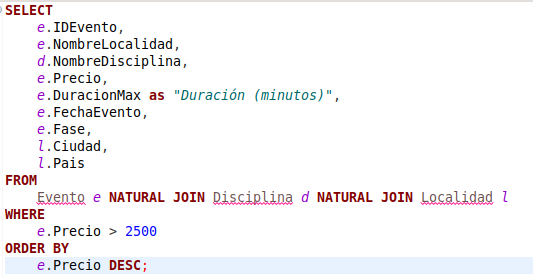
\includegraphics[width=10cm]{resources/consulta2.png}
\end{center}

Usamos join natural que solo esta en postgres:D

El resultado es:
\begin{center}
    
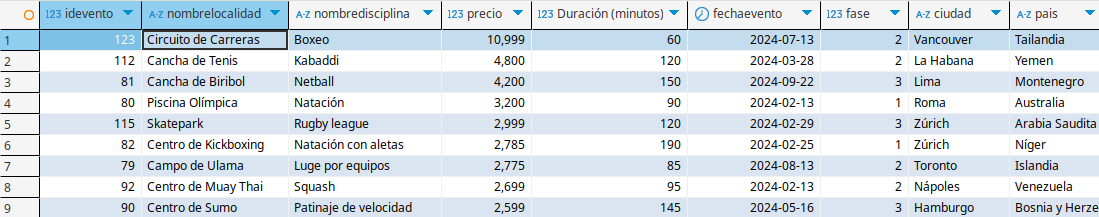
\includegraphics[width=15cm]{resources/consulta2.1.png}
\end{center}